%\subsection{\textit{Google Cloud Messaging}}

	\par O envio dos dados do \textit{web service} para o aplicativo
\textit{Android}, é feito através de um serviço da \textit{Google} conhecido
como GCM.

	\par Para que o serviço apresente o resultado esperado, foi preciso acessar o
\textit{site} da \textit{Google Developers Console} e criar um novo projeto. Ao
criá-lo, foi necessário ir na aba API's e ativar a opção \textit{Google Cloud
Messaging for Android}.

 	\par Com a criação do projeto, a \textit{Google} oferece um número que
identificará o \textit{software}, também chamado de \texttt{Sender ID},
conforme mostra a Figura \ref{fig:gcm}.


	\begin{figure}[h!] 
		\centerline{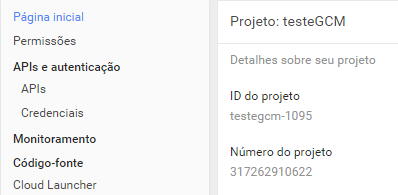
\includegraphics[scale=1]{./imagens/2_q_metodologico/4_procedimentos_resultados/41_gcm/gcm.png}}
		\caption[\texttt{Sender ID} do GCM]{\texttt{Sender ID} do GCM.
		\textbf{Fonte:}Elaborado pelos autores.}
		\label{fig:gcm}
	\end{figure}
	\pagebreak
	
	\par Por fim, acessou-se a aba Credenciais para indicar o IP do servidor. Ao
informa-lo, o serviço gerou uma chave pública a qual foi inserida no
\textit{web service}. Na Figura \ref{fig:gcm1}, é possível ver o código de
acesso criado.


	\begin{figure}[h!] 
		\centerline{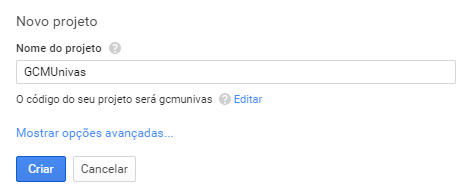
\includegraphics[scale=0.5]{./imagens/2_q_metodologico/4_procedimentos_resultados/41_gcm/gcm1.png}}
		\caption[Geração da credencial do GCM]{Geração da credencial do GCM.
		\textbf{Fonte:}Elaborado pelos autores.}
		\label{fig:gcm1}
	\end{figure}